\chapter{User Interface Design}
This chapter displays a more in depth analysis of the "3.1.1" section called "User Interface" of the
 Requirements Analysis and
 Specification Document (RASD) related to the S\&C project. 
 Within the scope of detail permitted in a design document, 
 it is possible to explore the various interactions the platform provides to external users,
  whether they are students or companies' authorized employees.
 The screenshots displayed in this section serve as mockups of the user interfaces provided by the system, 
 therefore they have to be interpreted as general guidelines for the designers and developers to
 grasp the application overall look at the end of the implementation process.

\newpage

\section{NavBar}
The navbar is the cardinal navigational component of the S\&C platform, 
designed to provide quick and intuitive access to the platform's core features. 
It features a minimalist, user-friendly design with the following icons:  

\begin{itemize}
    \item Messages: Provides access to the messaging interface, 
    allowing real-time communication between students and companies.  
    \item Inbox: Displays notifications, updates, 
    and invitations from companies or students in a streamlined format.  
    \item Search: Redirects to the Internship Browsing Page,
    enabling users to find internships, through either a keyword search or recommended hot topics.
    \item Profile: Takes users to their profile page, 
    where they can view and edit their information, CV, or internships offers (depending on the user).  
\end{itemize}
The navbar ensures a seamless user experience, remaining accessible across all pages of the platform.

\begin{figure} [H]
    \centering
    
\includegraphics [width=.1\linewidth] {ui1.png}
\end{figure}


\section{Login Page}
Login Page Description:
The login page serves as the primary gateway for users to access the S\&C platform. 
It features a clean and intuitive design to ensure a seamless user experience. 
The page includes the following key elements:

\begin{itemize}
    \item Username Field: a text input where users enter their username, checks the validity of the data entry.
    \item Email Field: A text input field where users enter their registered email address. 
    It validates the format to ensure correct data entry.
    \item Password Field: A secure input field for users to enter their password, with masking for privacy. 
    An optional "Show Password" "Hide" toggle enhances usability.
    \item Login Button: A button that, when clicked, authenticates the provided credentials 
    and, if correct, grants access to the platform. 
\end{itemize}

\begin{figure} [H]
    \centering
    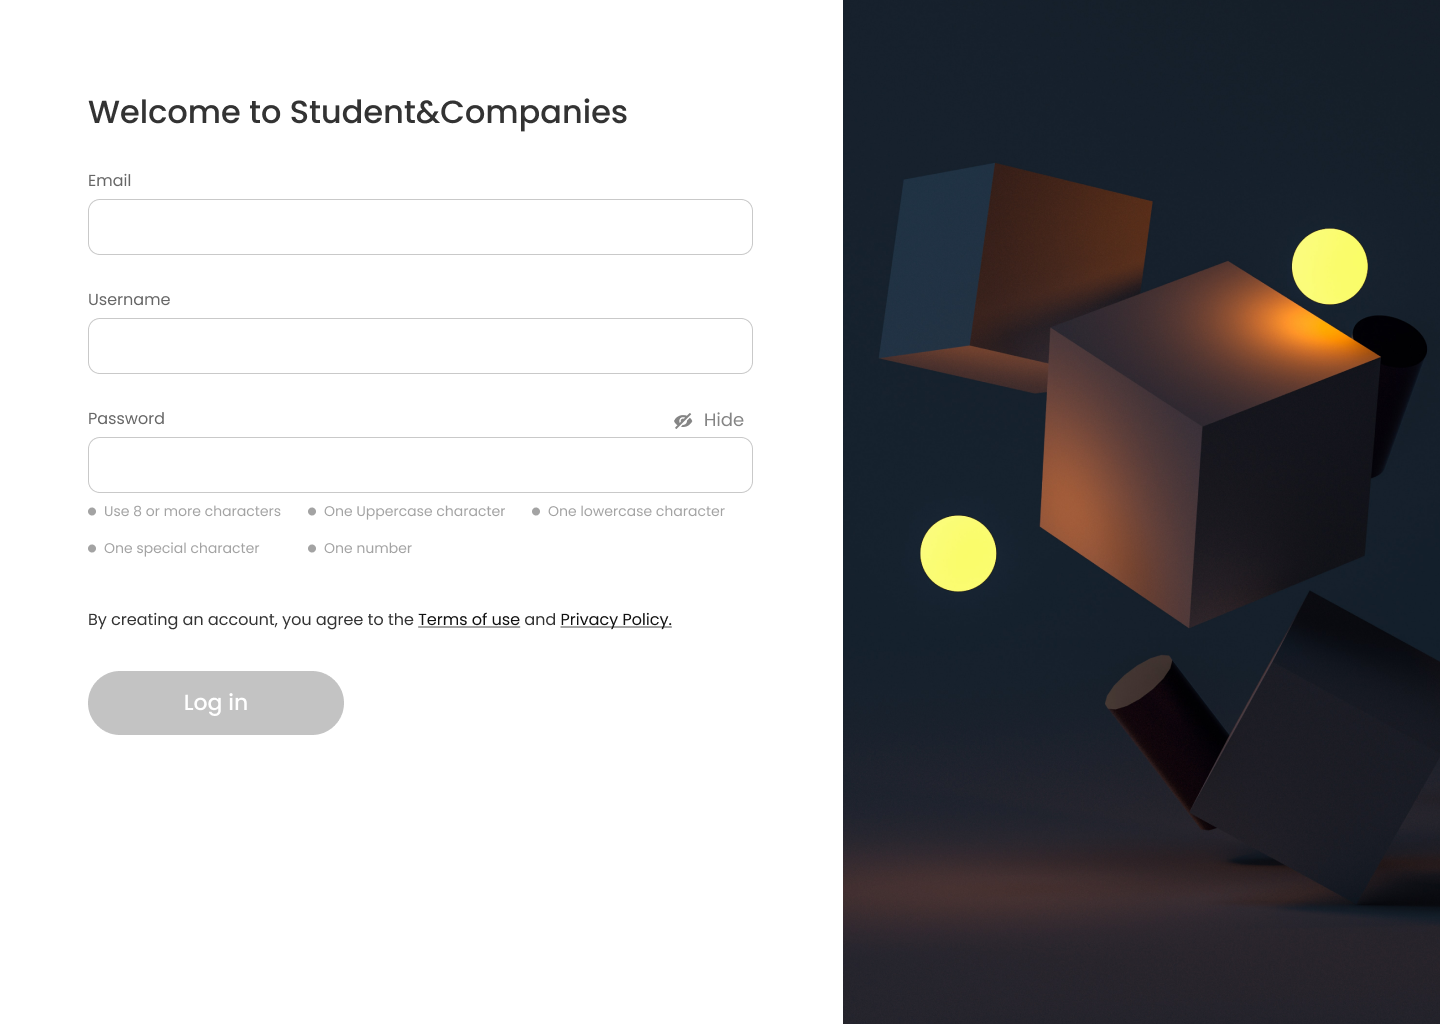
\includegraphics [width=.9\linewidth] {ui2.png}
\end{figure}


\section{Student Profile}
Student Profile:
The student profile page is designed to showcase a student's essential information 
in a structured and user-friendly manner. 
Each profile includes a customizable profile picture, along with the student’s email and phone number 
as primary contact details. A unique feature of the student profile is the inclusion of the university name 
at the bottom-right section, highlighting the institution the student is currently affiliated with. 
Additionally, along side a brief "about me" description, the page provides an option on the left side 
for users to download the student's CV directly, 
facilitating easy access to their qualifications and achievements.

\begin{figure} [H]
    \centering
    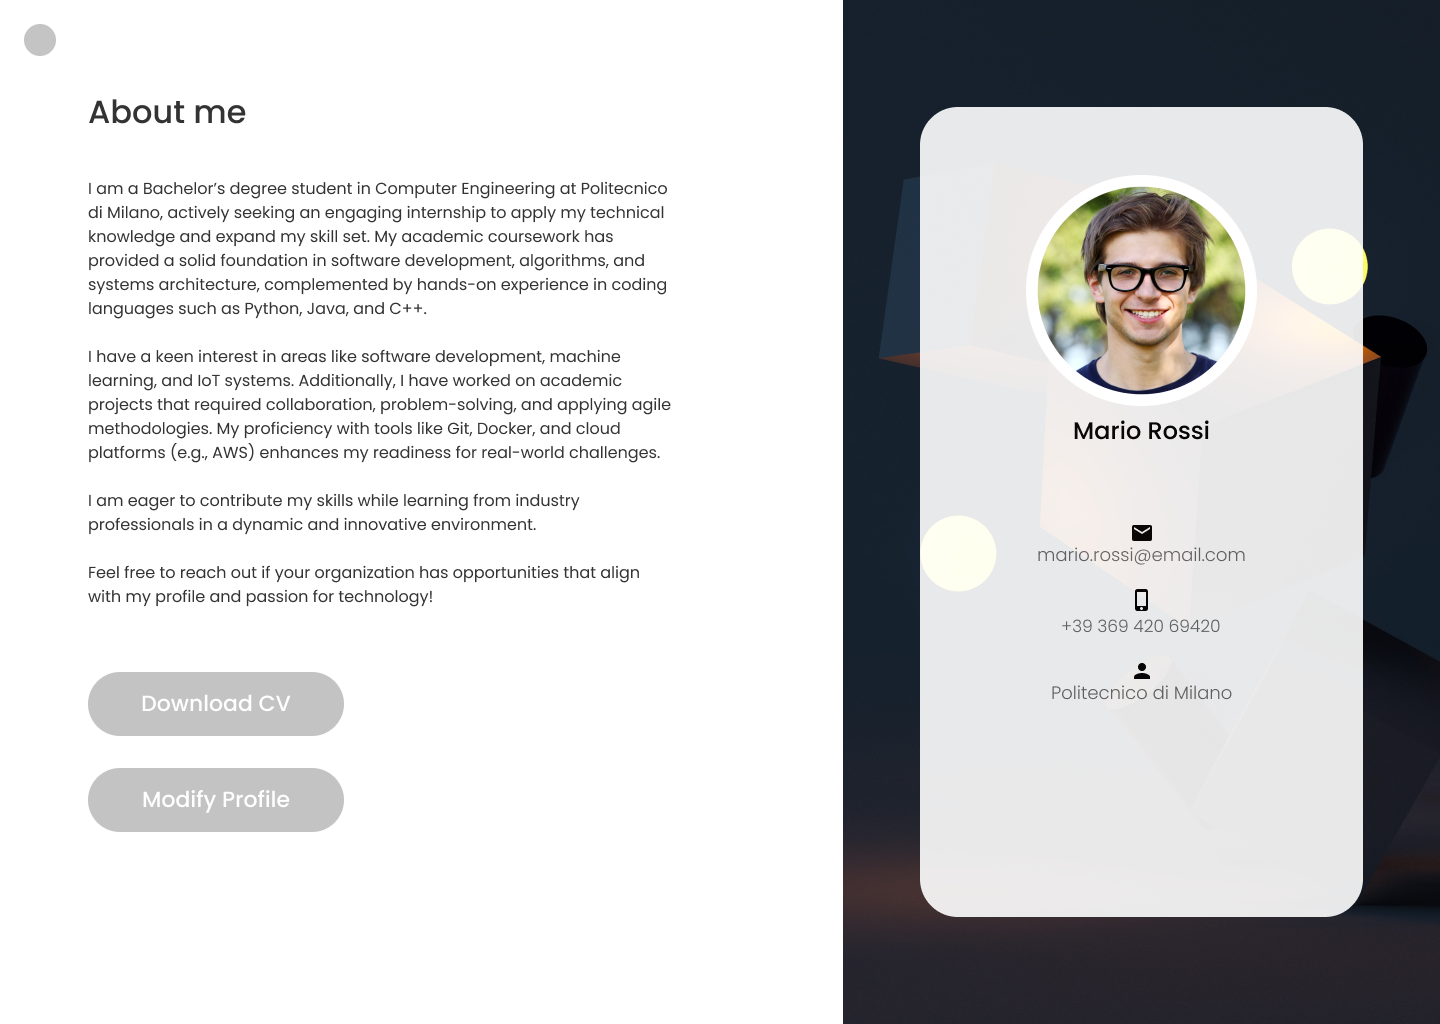
\includegraphics [width=.9\linewidth] {ui3.png}
\end{figure}

\newpage

\section{Company Profile}
The company profile page offers a professional overview of an organization, 
displaying its identity and opportunities. 
Similar to the student profile, it features a customizable profile picture, along with the company’s 
email and phone number for direct communication. 
Distinguishing itself from the student profile, the company page displays the name of
 its current CEO at the bottom-right section. On the left side, following an "about us" paragraph, the page provides a
  dedicated section to showcase the internships the company is currently offering, enabling students to explore potential
   opportunities with ease.

\begin{figure} [H]
    \centering
    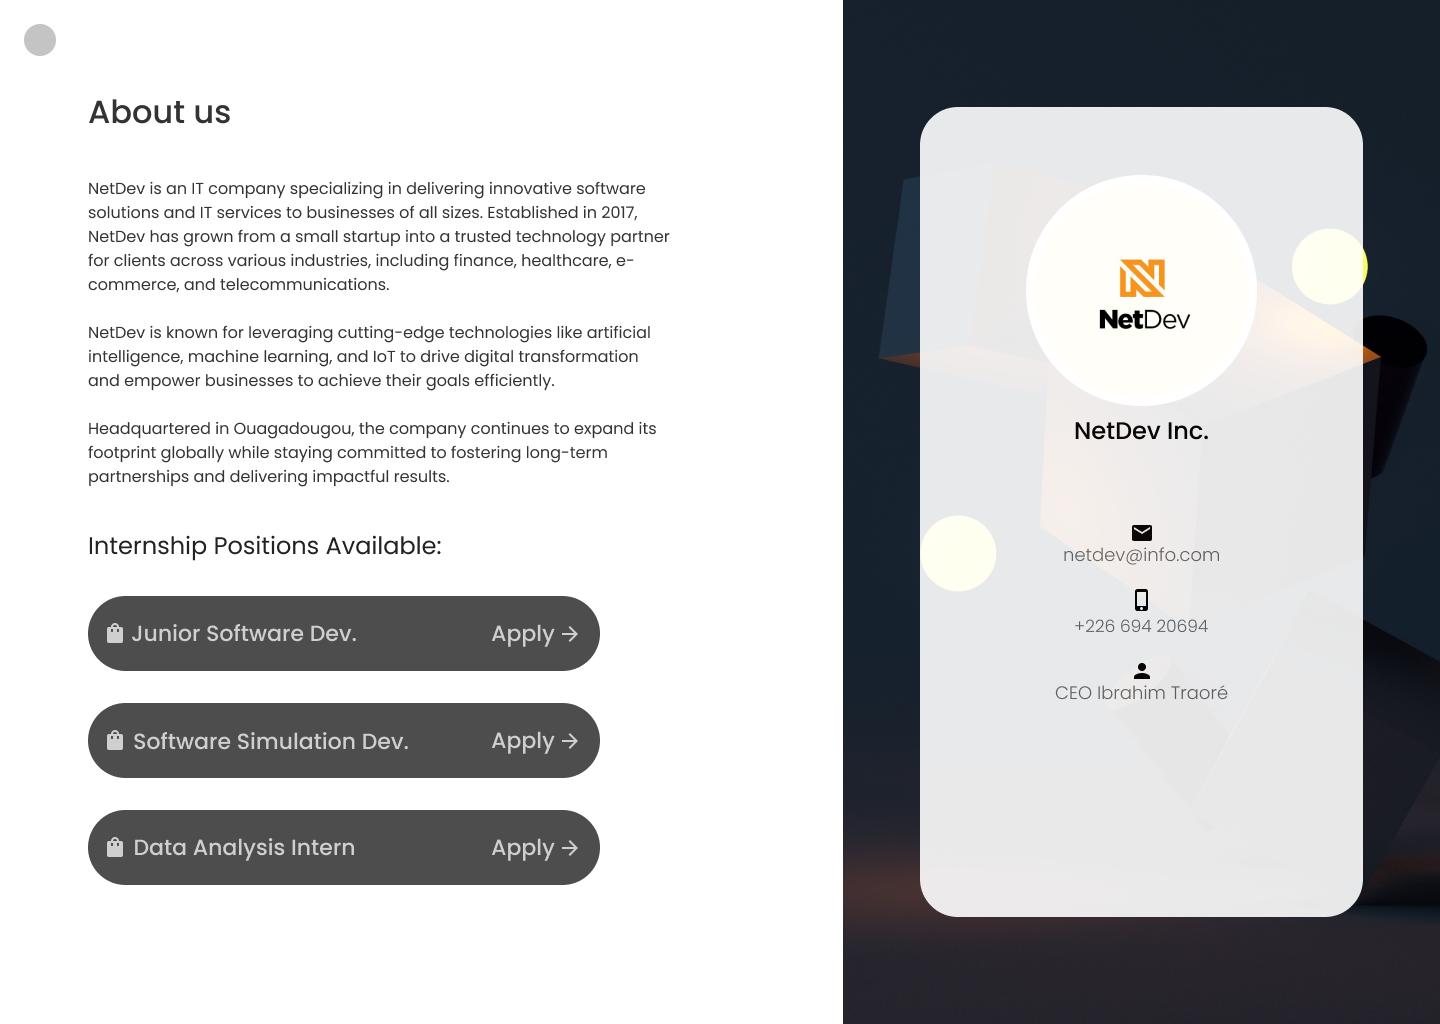
\includegraphics [width=.9\linewidth] {ui4.png}
\end{figure}   

\newpage

\section{Notification Inbox}
This section displays the list of notifications received by the system and potentially other users, 
the order in which are displayed is from the most recent one at the top to the least recent at the bottom.

\begin{figure} [H]
    \centering
    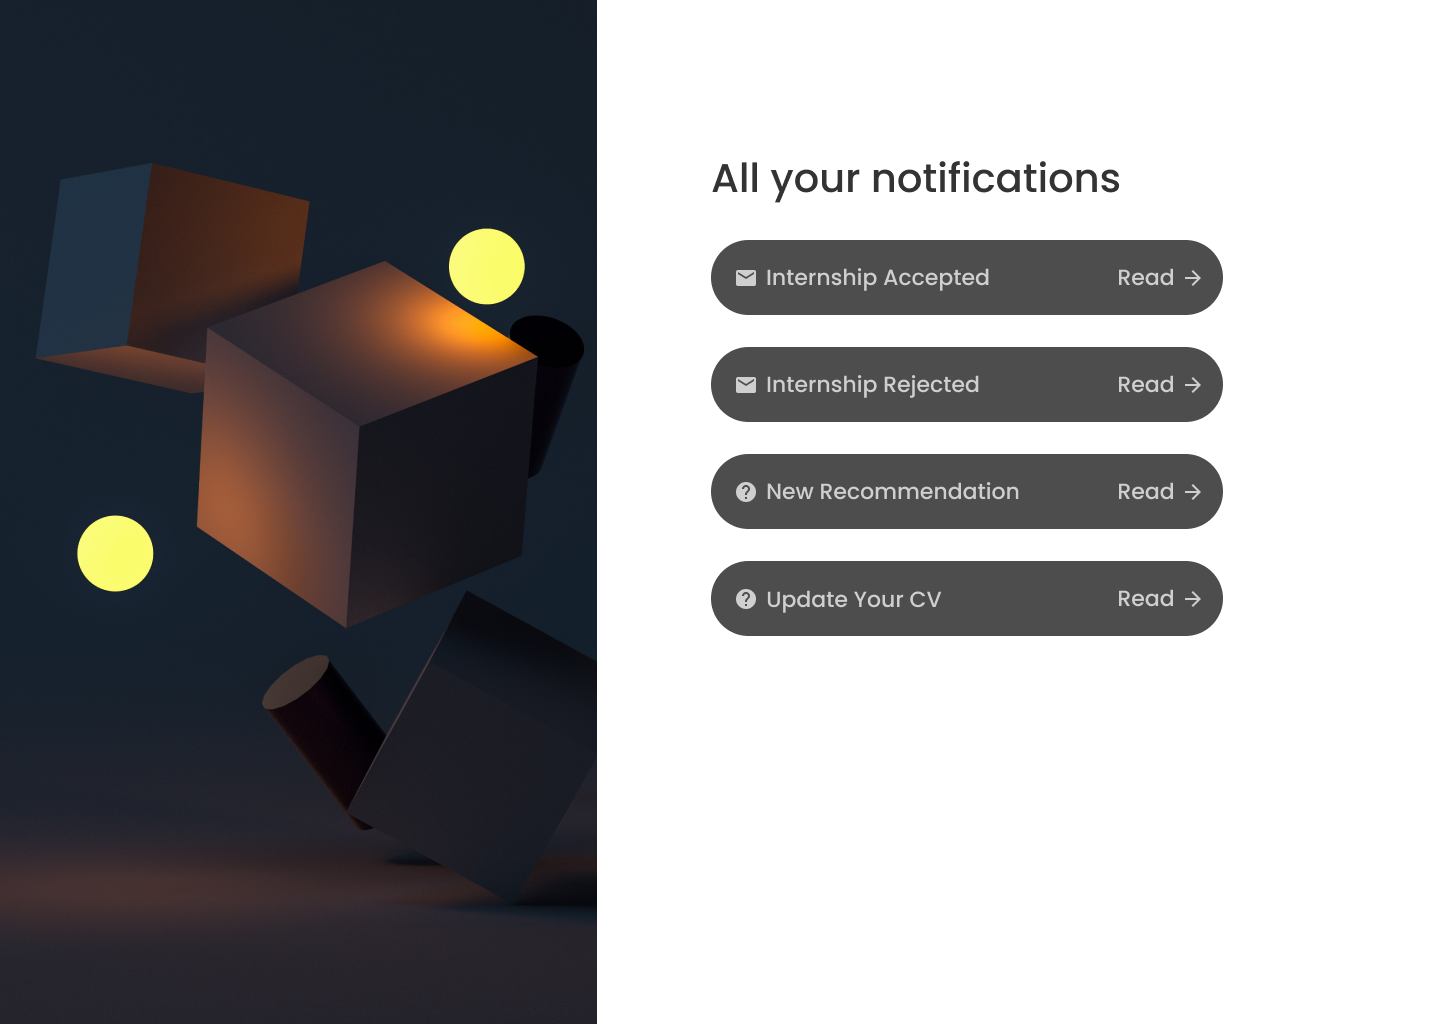
\includegraphics [width=.9\linewidth] {ui5.png}
\end{figure}

\newpage

\section{Internship Browsing Page}
The interface is divided in two main parts, on the right there is the search bar followed by the list of 
hot topics (internship related) of the current period, on the left there are the recommended internships available, 
sorted by the Recommendation Engine.

\begin{figure} [H]
    \centering
    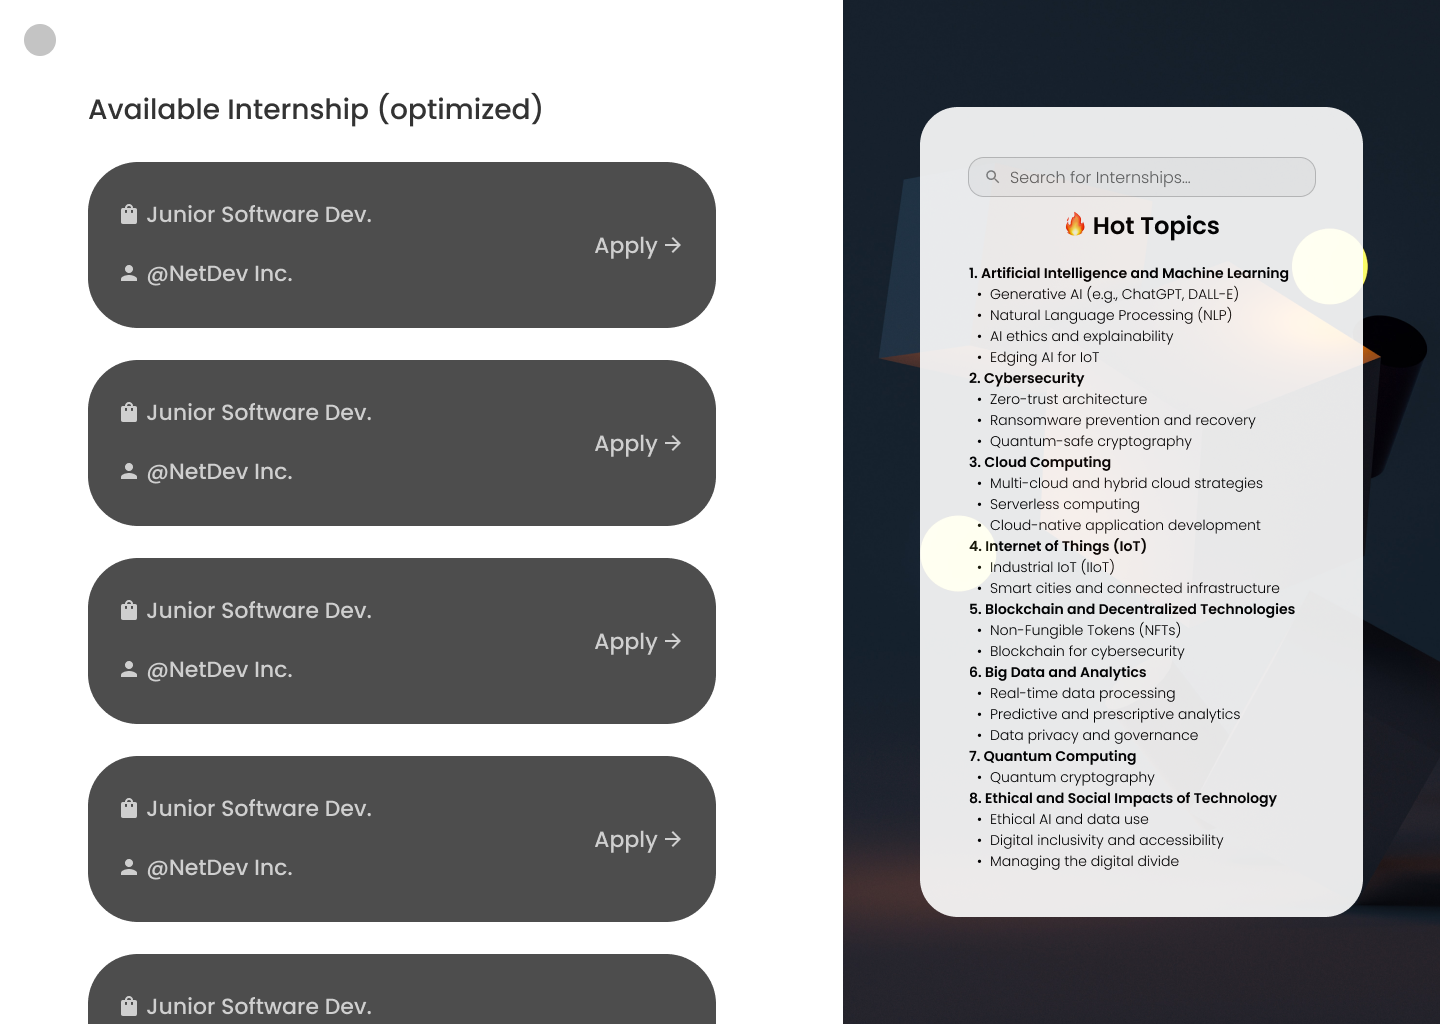
\includegraphics [width=.9\linewidth] {ui6.png}
\end{figure}

\newpage

\section{Internship Information Details}
In this page are displayed all the information regarding the selected internship, followed by the information 
about the company that is offering the position.
The button "Apply", once clicked, starts the application process.

\begin{figure} [H]
    \centering
    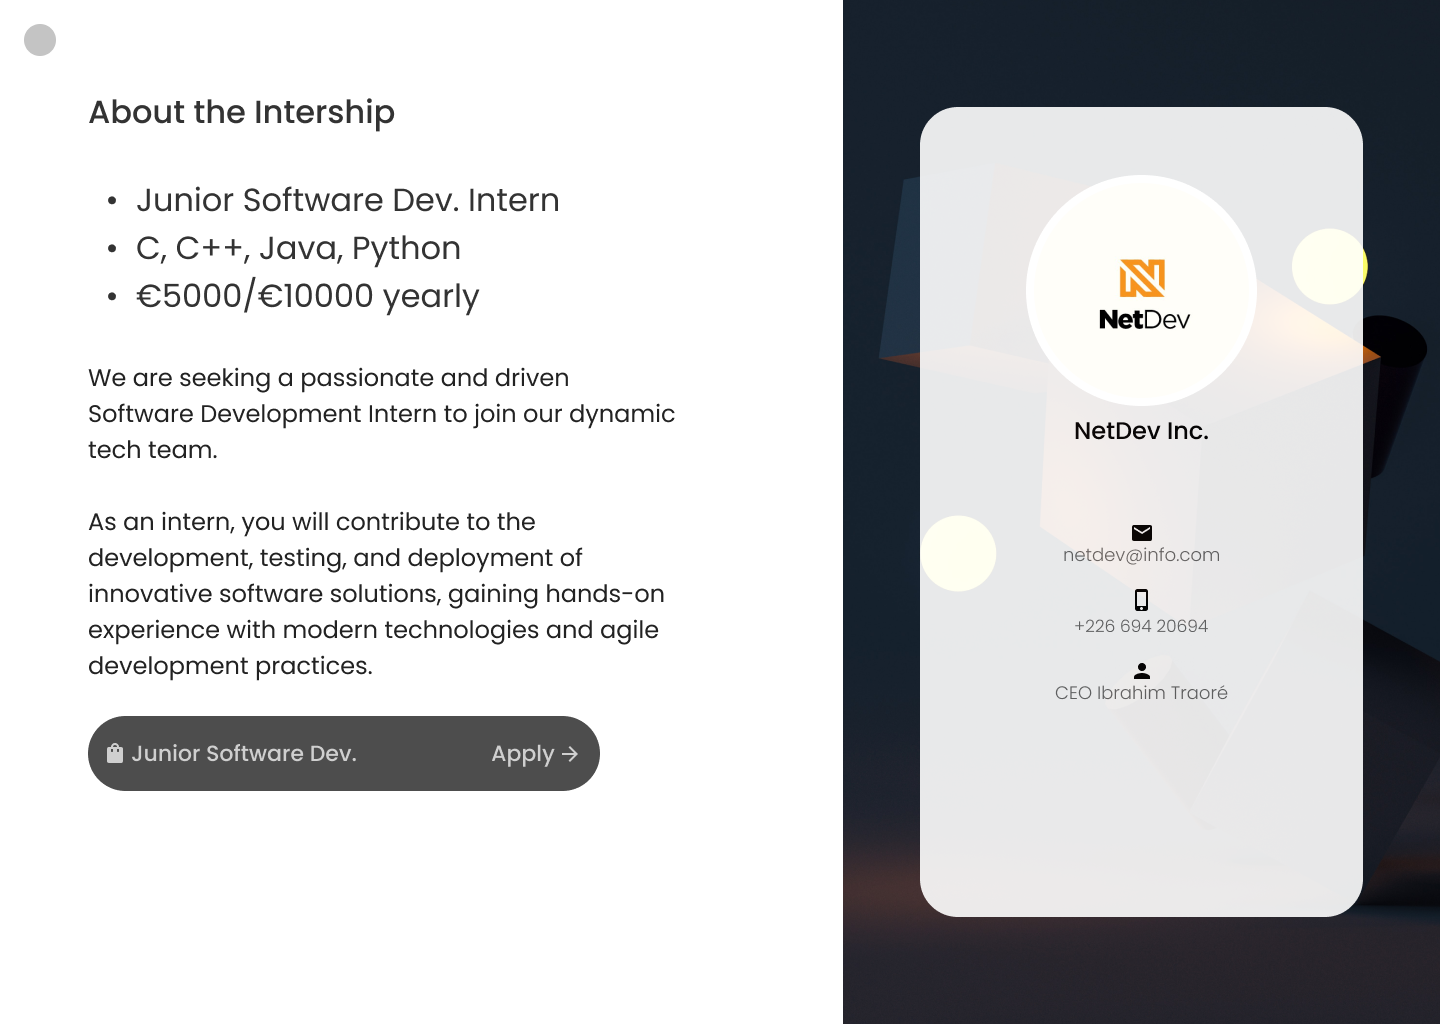
\includegraphics [width=.9\linewidth] {ui7.png}
\end{figure}

\newpage

\section{Chat}
The chat page is a streamlined interface designed for real-time communication between users. 
Key elements include:
\begin{itemize}
    \item Chat List: Displayed on the left side of the page, it shows a list of recent conversations, 
    including the name and profile picture of the other party.
    \item Chat Window: Occupying the main area of the page, 
    the chat window displays the active conversation in a chronological message thread. 
    \item Input Field: Located at the bottom of the chat window, the input field allows users to type messages. 
    Additional controls, send button and file attachment option, are present along side the text field.
    \item User Details: A small section or header that shows information about the chat participant, 
    such as their name, profile picture, and availability status.
    \item Team Members Section: Positioned to the side, this section lists all participants in the current conversation. 
    It displays their names, profile pictures, and role in the company, supporting easy identification and collaboration.
\end{itemize}

\begin{figure} [H]
    \centering
    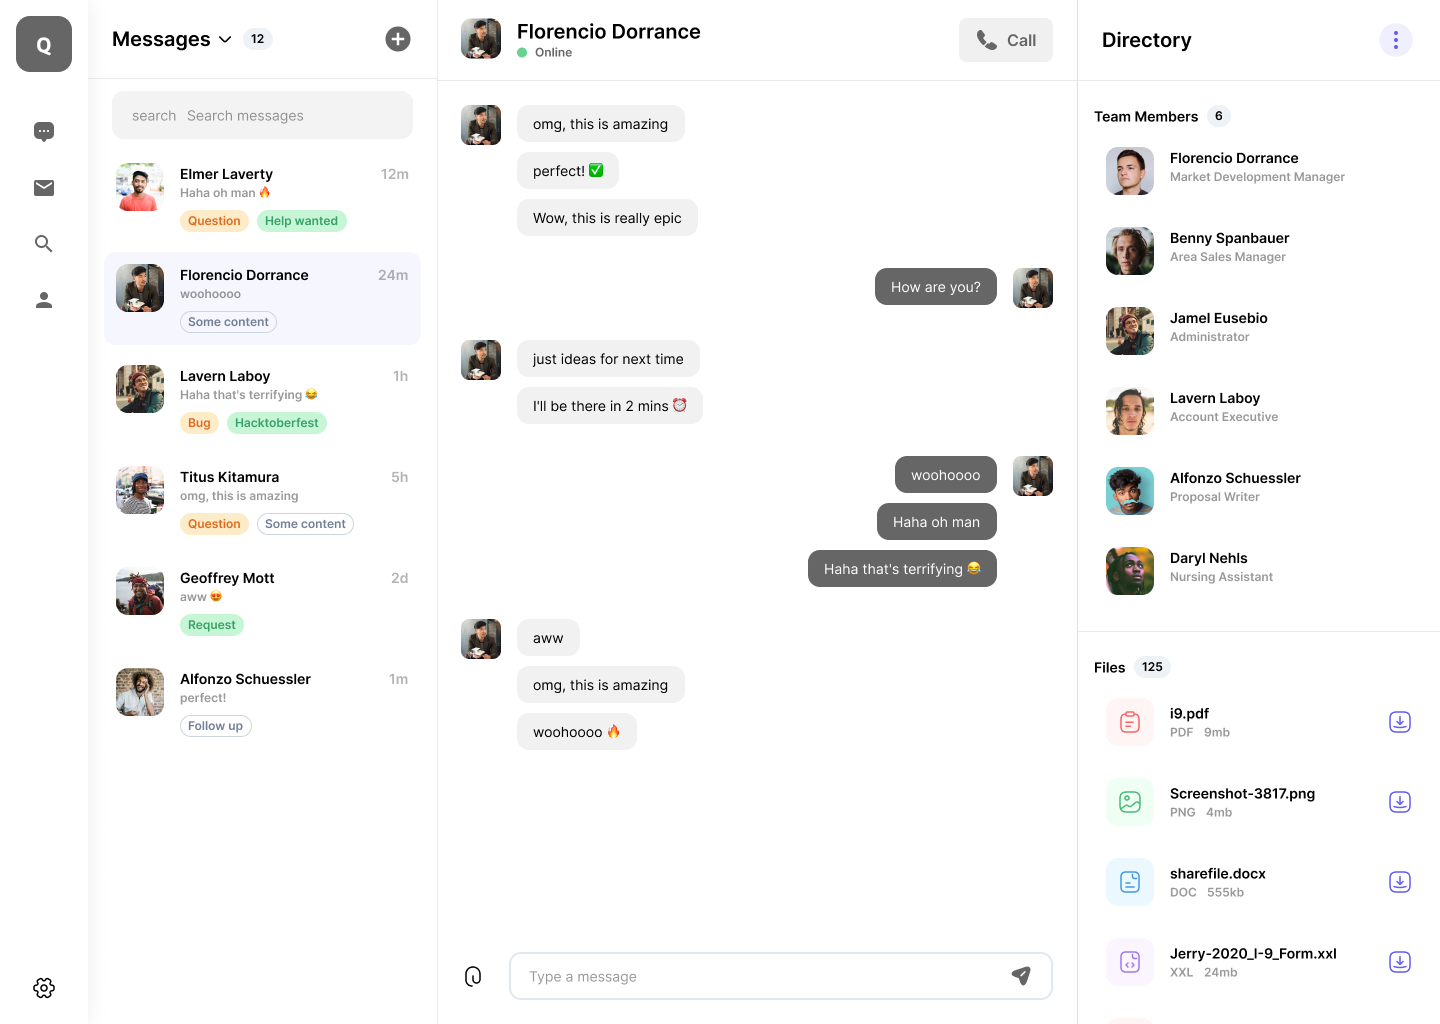
\includegraphics [width=.9\linewidth] {ui8.png}
\end{figure}

\newpage

\section{Feedback/Complaint}
This page contains a form used to send a formal complaint or give feedback directly to the S\&C platform itself.
It is divided in "About" drop list, "Parties involved" drop list, "Description" text field and at the bottom the "Send" button.

\begin{figure} [H]
    \centering
    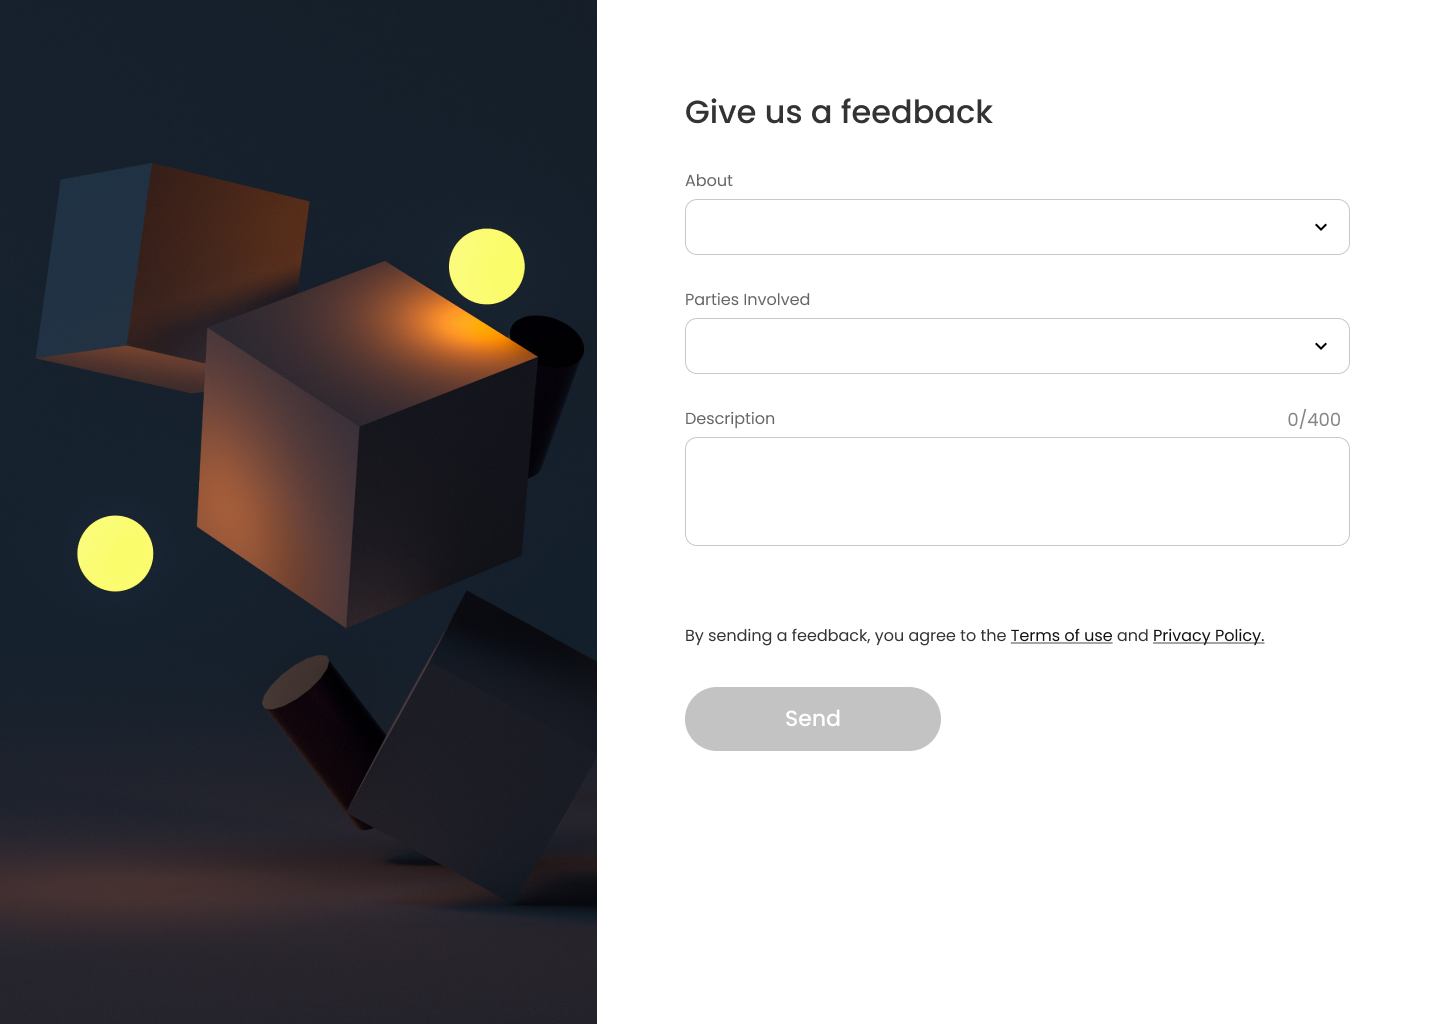
\includegraphics [width=.9\linewidth] {ui9.png}
\end{figure}

\newpage

\section{Internship Creation Form}
This page contains a form used by authorized companies to create an intership position in the S\&C platform.
It is divided in the following text fields: "Intership", "Minimum Requirements", "Sector", "Retribution", "Description" and
 at the bottom the "Create" button. 

 \begin{figure} [H]
    \centering
    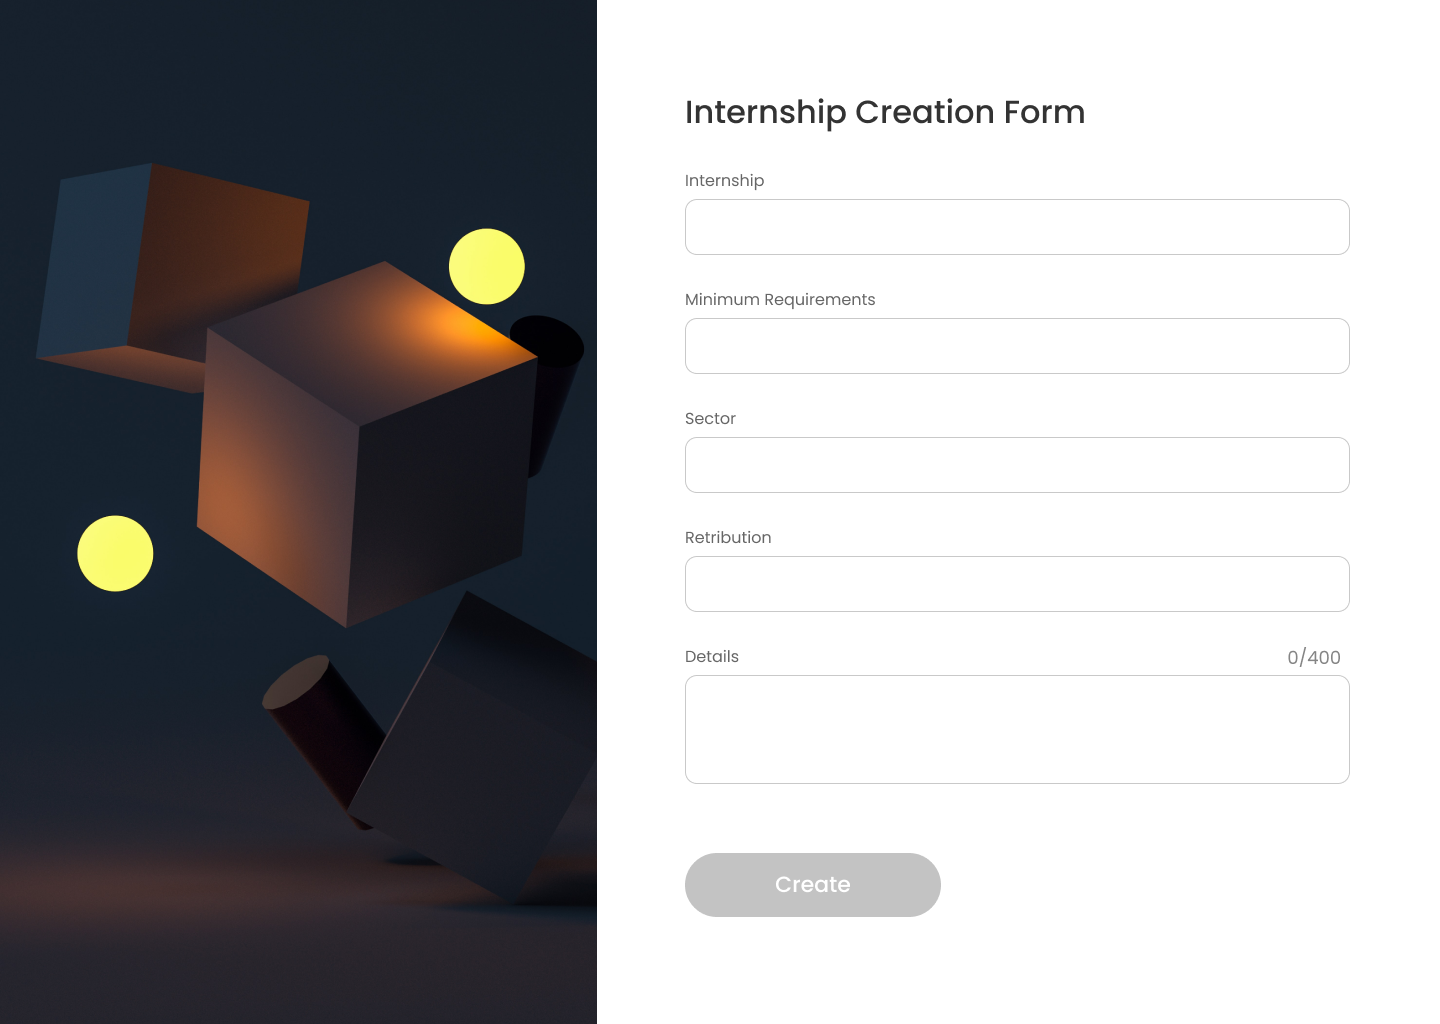
\includegraphics [width=.9\linewidth] {ui10.png}
\end{figure}


\newpage


\section{Preliminary Questionnaire}
This page contains a form required as a preliminary questionnaire at the beginning of the selection process.
It is divided in "Select your References" drop list, "Areas of expertise" drop list, "List of course" text field, 
"Technical skill set" text filed, "Description" text field and at the bottom the "Send" button.

\begin{figure} [H]
    \centering
    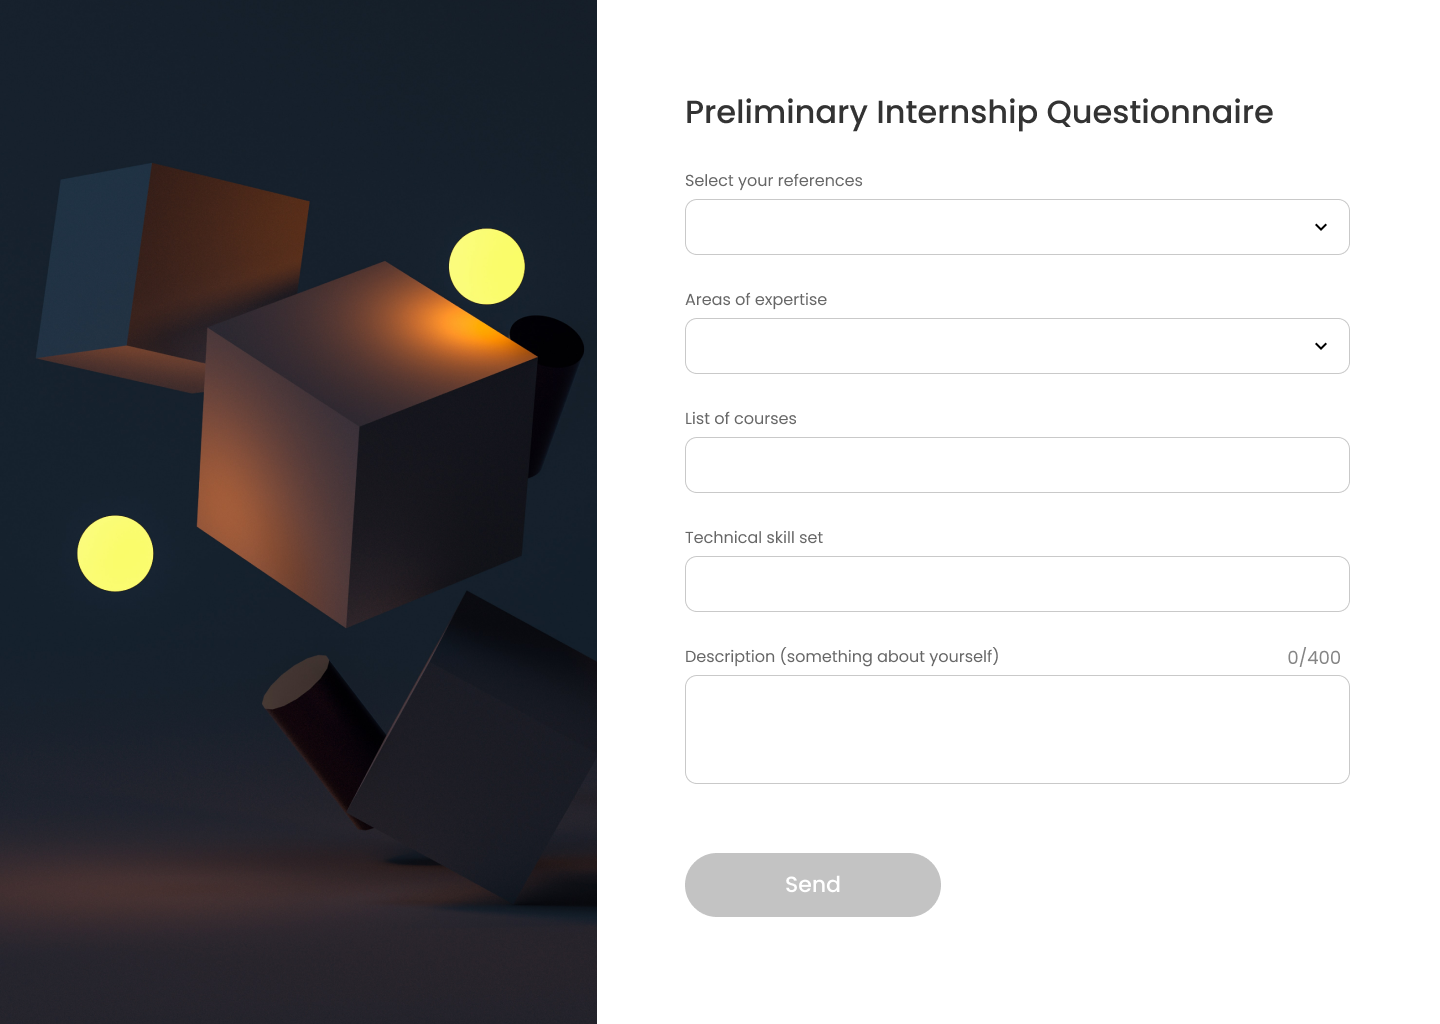
\includegraphics [width=.9\linewidth] {ui11.png}
\end{figure}


